\chapter{Termodynamikkens andre lov}

Som oftest tar vi det bare for gitt at varme naturlig strømmer fra et objekt med høy temperatur til et objekt med lav temperatur, og ikke omvendt. Faktisk kan man velge å definere temperatur som den egenskapen som lar oss forutsi hvilken retning varmestrømmen vil ha. Men hvis vi ser på objektene våre på et mikroskopisk nivå kan vi få en dypere forståelse av hvorfor energien strømmer den veien den gjør, og dette gir oss muligheten til å definere temperatur på en mer fundamental måte---og å få en av de dypeste innsiktene som ligger i termodynamikken.

\section{Mikrotilstander og makrotilstander}
Som nevnt i innledningen til denne teksten er grunntanken bak termodynamikken å beskrive et system med et sett av makroskopiske størrelser fordi en komplett mikroskopisk beskrivelse er praktisk umulig på grunn av det store antallet atomer. En tilstand som er beskrevet med unike verdier av disse makroskopiske størrelsene, f.eks. temperatur, trykk, volum og stoffmengde, kaller vi en \emph{makrotilstand}. Den fullstendige beskrivelsen av hvor hvert enkelt atom er og hvor fort det beveger seg kaller vi en \emph{mikrotilstand}. I alle realistiske scenarier vil det være et enormt antall mulige mikrotilstander for enhver makrotilstand. Sammen med termodynamikkens fundamentalpostulat---for et system i en gitt makrotilstand er alle mikrostilstander som er konsistent med denne makrotilstanden like sannsynlig---kan vi forstå hvorfor varme strømmer fra høy temperatur til lav temperatur. Dette gir oss også anledning til å innføre en ny fysisk størrelse som viser seg å være svært nyttig (men vanskelig å få helt taket på i første omgang): Entropi.

\subsection{Mikrotilstander i en enkel modell}
\label{sec:t2:minikrystall}
For å få en liten følelse for sammenhengen mellom mikrotilstander og makrotilstander kan det være godt med et konkret eksempel. Det viser seg at antall mikrotilstander vokser svært raskt med antall atomer i systemet, så vi holder det antallet lavt: Vi ser på en "krystall" som består av kun tre atomer. I følge kvantemekanikken kan atomene kun tildeles energi i faste kvanta---hvert atom kan ha enten \'en energienhet\footnote{Hvor stor energienheten er avhenger av hvilke atomer som er bundet sammen i krystallen. Størrelsen på energieheten er uansett uviktig for denne diskusjonen, det eneste som betyr noe er at energien er kvantisert.}, to energienheter, tre energienheter, osv. Hvis vi ikke plasserer noen energienheter på krystallen---svarende til den laveste temperaturen den kan ha---må nødvendigvis alle atomene være i tilstanden uten noen energienheter. Det er altså bare en måte å realisere dette på. Hvis vi øker temperaturen ørlite ved å plassere \'en energienhet på krystallen er det tre måter å realisere dette på: energienheten kan være på det første, det andre eller det tredje atomet. Jo flere energienheter vi plasserer på krystallen, jo flere mulige kombinasjoner finnes det som svarer til samme totalenergi. Tabell \ref{tab:t2:multipl} viser mulighetene for 0, 1, 2 og 3 energienheter.

\begin{table}[htp]
\begin{center}
\begin{tabular}{c|ccc}
& atom 1 & atom 2 & atom 3 \\
\hline
\hline
q = 0 & 0 & 0 & 0 \\
\hline
& 1 & 0 & 0 \\
q = 1 & 0 & 1 & 0 \\
& 0 & 0 & 1 \\
\hline
& 2 & 0 & 0 \\
& 0 & 2 & 0 \\
q = 2 & 0 & 0 & 2 \\
& 1 & 1 & 0 \\
& 1 & 0 & 1 \\
& 0 & 1 & 1  \\
\hline
& 3 & 0 & 0 \\
& 0 & 3 & 0 \\
& 0 & 0 & 3 \\
& 2 & 1 & 0 \\
q = 3 & 2 & 0 & 1 \\
& 1 & 2 & 0 \\
& 0 & 2 & 1  \\
& 1 & 0 & 2 \\
& 0 & 1 & 2 \\
& 1 & 1 & 1 \\
\hline
\hline
\end{tabular}
\end{center}
\caption{Mikrotilstander for en krystall med $N=3$ atomer og $q = 0, 1, 2$ eller 3 energienheter.}
\label{tab:t2:multipl}
\end{table}

Generelt kan det vises at antall mikrotilstander på en krystall med $N$ atomer og $q$ energienheter er 
\begin{displaymath}
	\Omega = \frac{(q+N-1)!}{q!(N-1)!}.
\end{displaymath}
For et makroskopisk objekt vil $N$ være av størrelsesorden $10^{23}$, og for temperatur omkring romtemperatur vil $q$ være vesentlig større enn dette. Det er derfor opplagt at antall mikrotilstander i et makroskopisk objekt er svært stort. 

\section{Entropi}
\label{sec:t2:entropi}
Blant annet fordi antall mikrotilstander vokser så raskt med når antall atomer og antall energienheter vokser er det mer hensiktsmessig å regne med $\ln\Omega$ enn $\Omega$ selv. Dette gjør at vi får tall av langt mer håndterbar størrelse, og som vi skal se snart har det også det å regne med logaritmen av antall tilstander en annen svært nyttig egenskap. Av historiske årsaker er det også vanlig å multiplisere $\ln\Omega$ med Boltzmanns konstant\footnote{Ved å ta med denne konstanten blir denne definisjonen av entropi kompatibel med entropi-definisjonen som var i bruk før mikro-fysikken som lå bak var forstått.}, $k=1,38\times10^{-23}~\mathrm{J/K}$. Vi får da størrelsen som har navnet \emph{entropi}:
\begin{displaymath}
	S = k\ln\Omega.
\end{displaymath}
Entropi er et slags kvalitetsmål til energien i systemet. Hvis entropien er lav kan energien i stor grad utnyttes til det vi måtte ønske å gjøre med den, mens jo høyere entropien blir, jo mindre blir muligheten til å anvende energien til å få gjort noen form for arbeid. Det ekstreme tilfellet er når alt i universet en gang i fjern fremtid har samme temperatur: Da er entropien maksimert og ingenting interessant kan lenger hende.

Entropi er i likhet med for eksempel indre energi, temperatur og trykk en tilstandsvariabel. Det vil si at hvis vi skal spesifisere tilstanden til et system fullstendig er entropien en av variablene som må oppgis.\footnote{Entropien er selvfølgelig ikke uavhengig av de andre tilstandsvariablene. For eksempel er entropien til en ideell gass unikt spesifisert dersom vi kjenner gassens volum, stoffmengde, masse per molekyl og indre energi.} Her kommer vi tilbake til hvorfor logaritmen er nyttig: Anta at vi har et system som består av to deler, kall de del A og del B. La del A ha $\Omega_A$ antall mikrotilstander og del B $\Omega_B$ antall mikrotilstander. Totalt antall mikrosystemer til systemet er da $\Omega = \Omega_A\cdot\Omega_B$. Ved å bruke regnereglene for logaritmer finner vi da ut at 
\begin{displaymath}
	S = k\ln\Omega = k\ln(\Omega_A\cdot\Omega_B) = k\ln\Omega_A + k\ln\Omega_B = S_A + S_B.
\end{displaymath}
Vi ser altså at på grunn av logaritmen i entropidefinisjonen er entropien til et system lik summen av entropien til alle delene av systemet, på akkurat samme måte som at indre energi til systemet er lik summen av indre energi til alle delene av systemet. 

\section{Mikrotilstander og temperatur}
Det er et aspekt ved entropien som er svært ulik andre tilstandsvariabler: Entropien til et isolert system avtar aldri, men den kan vokse. Dette viser seg å være tett koblet til observasjonen at varme flyter fra objekter til høy temperatur til objekter med lav temperatur. For å se denne sammenhengen skal vi se på et system som er satt sammen av to slike mini-krystaller som ble diskutert i avsnitt \ref{sec:t2:minikrystall}. Vi lar de to krystallene være i kontakt slik at de kan utveksle energi innbyrdes, mens de er isolert fra alt annet. Temperaturen til hver av krystallene er bestemt av energiinnholdet den har til enhver tid. Siden krystallene er like vil da lik temperatur hver ensbetydende med at energien er like fordelt mellom dem.

Hver krystall består av tre atomer, altså er $N_A = N_B = 3$. Vi lar $q_A$ og $q_B$ være antall energienheter på de to krystallene, og vi ser på tilfellet der $q_A + q_B = 6$. Siden energien kun kan utveksles mellom de to krystallene og ikke med omgivelsene vil denne summen holde seg konstant selv om $q_A$ og $q_B$ kan endres. Tabell \ref{tab:t2:multipl2} lister opp antall tilgjengelige tilstander i krystall $A$ og krystall $B$ gitt hver av de mulige verdiene til $q_A$ og $q_B$. Siden måten energien er fordelt mellom de ulike atomene i krystall $A$ er uavhengig av måten energien er fordelt mellom atomene i krystall $B$ er totalt antall mulige tilstander for en viss kombinasjon av $q_A$ og $q_B$ lik produktet av antall mulige tilstander i hver av krystallene, $\Omega_\text{tot} = \Omega_A\cdot\Omega_B$. Siste kolonne viser hvor stor andel av antall totalt mulig antall kombinasjoner som utgjøres av hver spesfikke kombinasjon av  $q_A$ og $q_B$. På grunn av antakelsen om at alle mikrotilstander som svarer til samme makrotilstand er like sannsynlig svarer dette forholdstallet til sannsynligheten for at akkurat denne kominasjonen av $q_A$ og $q_B$ realiseres.\footnote{Vi snakker her hele tiden om hvilken tilstand systemet er i etter at det har gått lang nok tid til å ha nådd termisk likevekt. Hvis vi ser på kortere tidsskalaer vil en mikrotilstand som ligner den forrige være mer sannynlig enn en som er mer ulik den forrige.}

\begin{table}[htp]
\begin{center}
\begin{tabular}{rr|rr|r|r}
$q_A$ & $\Omega_A$ & $q_b$ & $\Omega_B$ & $\Omega_\text{tot}$ & $P(q_A,q_B)$ \\ 
\hline
0 & 1 & 6 & 28 & 28 & 6,1\% \\
1 & 3 & 5 & 21 & 63 & 13,6\% \\
2 & 6 & 4 & 15 & 90 & 19,5\%\\
3 & 10 & 3 & 10 & 100 & 21,6\% \\
4 & 15 & 2 & 6 & 90 & 19,5\% \\
5 & 21 & 1 & 3 & 63 & 13,6\% \\
6 & 28 & 0 & 1 & 28 & 6,2\% \\
\end{tabular}
\end{center}
\caption{Antall mikrotilstander for hver makrotilstand gitt $N_A = N_B = 3$ og $q_A + q_B=6$. }
\label{tab:t2:multipl2}
\end{table}

Som tabellen viser er det komibinasjonen der $q_A = q_B$ som har flest tilgjengelige mikrotilstander. Dette er derfor den makrotilstanden vi må forvente at krystallen er i etter at det har gått lang tid. Hvis vi for eksempel starter opp med all energien på krystall A, altså $q_A = 6$, må vi forvente at energien fordeler seg jevnt utover slik at halvparten av energien etter hvert havner på krystall $B$---vi ender altså opp med at krystallene som startet med ulik temperatur til slutt får lik temperatur.

I dette eksempelet er det ikke stor forskjell i sannynlighet selv mellom tilstander som har ganske ulike energifordeling. Om vi sammenligner tilstanden med $q_A=2, q_B=4$ og $q_A = q_B = 3$ er førstnevnte tilstand kun 10\% mindre sannsynlig selv om krystall B i dette tilfellet har dobbelt så mye energi som krystall $A$. Dette er en artefakt av at eksempel-systemet vårt er så lite. Hvis vi ser på et reelt system med $N$ omkring $10^{23}$ og $q$ enda større enn dette ender vi opp med en sannsynlighetsfordeling som har en svært smal topp rundt den mest sannsynlige energifordelingen. Selv svært små avvik ender opp med forsvinnende liten sannsynlighet.

\begin{figure}[tp]
\begin{center}
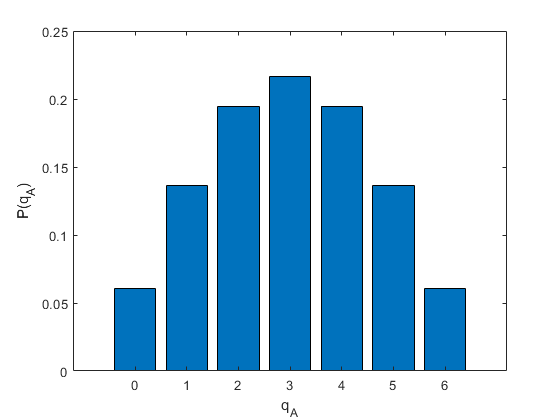
\includegraphics[width=.45\textwidth]{./multiplisitet_3_3_6}
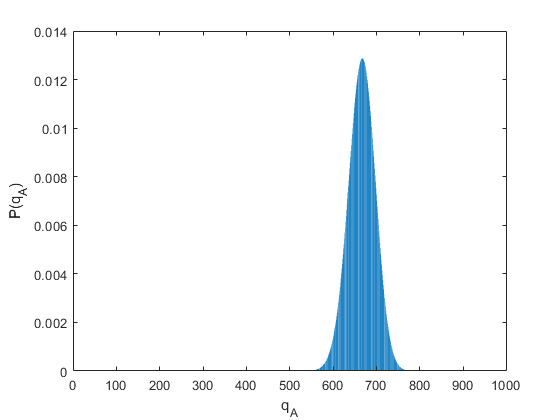
\includegraphics[width=.45\textwidth]{./multiplisitet_200_100_1000}
\end{center}
\caption{Sannsynlighetsfordeling for ulike verdier av $q_A$. I plottet til venstre er $N_A = N_B = 3$ og $q_A + q_B = 6$. I plottet til høyre er $N_A = 200, N_B=100$ og $q_A + q_B = 1000$. Selv om størrelsen på antall atomer og antall energienheter i plottet til høyre fremdeles er mye mindre enn i realistiske eksempler ser vi at et kun er energifordelinger nær den mest sannsynlige verdien som har sannsynlighet vesentlig større enn 0. Når $N$ og $q$ blir store nok til å representre et realisitisk makroskopisk system blir toppen mye smalere. Merk også at i plottet til høyre er det $q_A = \frac{2}{3}(q_A+q_B)$ som er mest sannsynlige verdi siden $N_A = 2N_B$. }
\label{fig:t2:multiplisitet}
\end{figure}

En variasjon av eksempelet ovenfor som også er interessant å se på er å la de to krystallene ha ulik størrelse, f.eks. $N_A = 5, N_B = 3$. Hvis vi gjør tilsvarende beregning som i tabell \ref{tab:t2:multipl2} for det tilfellet vil vi naturlig nok finne at det ikke er lik energifordeling mellom de to krystallene som er mest sannsynlig. Vi finner derimot at det er mest sannsynlig at krystall A har $\frac{5}{5+3}\cdot100\% = 62,5\%$ av energien mens krystall B har de resterende 37,5\% av energien. Beregningen viser altså at tilstanden med like stor energi\emph{tetthet} er den mest sannsynlige, og temperatur beskriver nettopp energitetthet og ikke totalt energiinnhold. 

Eksemplene i dette avsnittet viser at tendensen til utgjevning av energitetthet, og dermed temperatur, kan forstås ved å se på antall tilgjengelige mikrotilstander for de ulike makrotilstandene. Neste avsnitt vil ta denne konklusjonen videre og formulere den ved hjelp av størrelsen entropi som ble definert i avsnitt \ref{sec:t2:entropi}.

\section{Entropi og temperatur}
Diskusjonen i forrige avsnitt viste at energien i et isolert system vil fordele seg slik at systemet ender opp i den makrotilstanden med flest tilhørende mikrotilstander. Siden logaritmen er er en monotont økende funksjon er dette ekvivalent med å si at systemet ender opp i den makrotilstanden der entropien, $S = k\ln\Omega$ er størst. Hvis vi fortsetter å betrakte et system som består av delsystemene A og B (ikke nødvendigvis like store) kan vi da skrive likevektskriteriet
\begin{equation}
	\frac{\partial S_\text{total}}{\partial U_A} = 0.
	\label{eq:t2:likevekt1}
\end{equation}
Her er $U_A$ den indre energien i delsystem A. Diskusjonen i forrige avsnitt var basert på antall energienheter i delsystemet, $q_A$, men siden $U_A = \epsilon q_A$ der $\epsilon$ er en konstant kan vi like gjerne uttrykke likevektsvilkåret i form av $U_A$. Videre er hver enkelt energienhet svært liten sammenlignet med den totale indre energien for et makroskopisk system. Derfor er det helt greit å behandle $U_A$ og $S$ som kontinuerlig varierende størrelser slik vi implisitt har gjort ved å skrive ned den deriverte.

Når vi skal jobbe videre med dette uttrykket husker vi på at $S_\text{total} = S_A + S_B$. Videre må enhver endring i $U_A$ kompenseres med en like stor endring med motsatt fortegn i $U_B$ siden vi har antatt at systemet som helhet er isolert fra omgivelsene. Derfor kan ligning (\ref{eq:t2:likevekt1}) omskrives som
\begin{displaymath}
	0 = \frac{\partial S_\text{total}}{\partial U_A} = \frac{\partial S_A}{\partial U_A} + \frac{\partial S_B}{\partial U_A}
	 = \frac{\partial S_A}{\partial U_A} - \frac{\partial S_B}{\partial U_B}
\end{displaymath}
eller
\begin{displaymath}
	\frac{\partial S_A}{\partial U_A} = \frac{\partial S_B}{\partial U_B} \quad \text{(ved likevekt)}.
	\label{eq:t2:likevekt2}
\end{displaymath}
Venstresiden av denne ligningen sier noe om bare delsystem A, mens høyre\-siden sier noe om bare delsystem B. Dette tyder på at størrelsen $\partial S/\partial U$ kan brukes til å karakterisere en bestemt del av et system. Videre sier ligning (\ref{eq:t2:likevekt2}) at denne størrelsen er lik i ulike deler av systemet når det har kommet i likevekt. Dette ser lovende ut som et mål på temperatur. Som et neste steg ser vi på enhetene: Entropi har enhet $\mathrm{J/K}$, mens energi har enhet $\mathrm{J}$. Dermed har $\partial S/\partial U$ enhet $\mathrm{K^{-1}}$. Enhetene tyder derfor på at temperatur kan uttrykkes som 
\begin{equation}
	T = \left(\frac{\partial S}{\partial U}\right)^{-1}.
	\label{eq:t2:T}
\end{equation}
Siden dette argumentet fremkom delvis gjennom kvalitative argumenter og delvis dimensjonsanalyse kan vi i utgangspunktet ikke utelukke at det skal være noen konstantfaktorer, f.eks. en faktor 2 eller $\pi$, med i dette uttrykket. Jeg skal ikke forsøke å vise her at det ikke er behov for noen slike faktorer, men bare konstantere at temperaturen definert gjennom ligning (\ref{eq:t2:T}) er konsistent med temperaturdefinisjonen som er brukt tidligere i teksten.

\section{Entropi og varmeoverføring}
Som en avslutning på diskusjonen om temperatur og entropi ser vi nå på varmeoverføring mellom to makroskopiske objekter med starttemperatur henholdsvis $T_1$ og $T_2$. Vi begrenser oss til å se på et tilfelle der det ikke utføres noe arbeid samtidig som varmefoverføringen, og det er ingen energiutveksling mellom omgivelsene. Da er $\Delta U = Q$ for hvert av objektene, og $Q_1 = -Q_2$. Hvis vi antar at objekt 2 har lavest temperatur vil dette motta energi og følgelig er $Q_2$ positiv.

Vi kan bruke ligning (\ref{eq:t2:T}) individuelt for hvert av objektene. Hvis vi i første omgang begrenser oss til å se på infinitesimale endringer gir denne:
\begin{align*}
	\d S_1 &= \frac{\d U_1}{T} = \frac{\d Q_1}{T} = m_1c_V\frac{\d T}{T}\\
	\d S_2 &= \frac{\d U_2}{T} = \frac{\d Q_2}{ T}= m_2c_V\frac{\d T}{T} \\
\end{align*}
Her er $T$ dent temperaturen objektet har til enhver tid (kun samme verdi for begge objekter når de har kommet i termisk likevekt). Den siste likheten følger av definisjonen for varmekapasitet, samt at prosessen må skje ved konstant volum siden vi har antatt at det ikke blir utført noe mekanisk arbeid. For å finne total endring av entropi integrerer vi disse uttrykkene fra starttemperaturen, henholdsvis $T_1$ og $T_2$ til den felles temperaturen de har når de er kommet til termisk likevekt, $T_f$. 
\begin{align*}
	\Delta S_1 &= m_1c_V\int_{T_1}^{T_f} \frac{\d T}{T} = m_1c_V\ln\left(\frac{T_f}{T_1}\right) = - m_1c_V\ln\left(\frac{T_1}{T_f}\right), \\
	\Delta S_2 &= m_2c_V\int_{T_2}^{T_f} \frac{\d T}{T} = m_2c_V\ln\left(\frac{T_f}{T_2}\right).
\end{align*}
Siden $T_1 > T_f > T_2$ er $\Delta S_1$ negativ, mens $\Delta S_2$ er positiv. Hvis vi summerer disse finner vi at $\Delta S_\text{total} = \Delta S_1 + \Delta S_2>0$ uansett hva forholdet mellom $m_1$ og$m_2$ er, og uansett om de to objektene har samme verdi for $c_V$ eller ikke. Dette kan vi enklest se ved å sammenligne uttrykkene for $\d S_1$ og $\d S_2$. Siden de kun utveksler energi med hverandre og ikke med øvrige omgivelser må $|\d Q_1| = |\d Q_2|$ til enhver tid. Men fordi objekt 1 starter på en høyere temperatur enn objekt 2 er temperaturen i nevneren for $\d S_1$ alltid større eller lik den i nevneren for $\d S_2$. Dermed er til enhver tid $|\d S_2|\geq |\d S_1|$. Vi ser altså at entropiøkningen i objektet som mottar energi nødvendigvis er større enn entropireduksjonen i objektet som mottar energi. Nettoresultatet er at den totale entropien øker.

 De eneste prosessene som kan unngå å øke den totale entropien er adiabatiske prosesser---der det ikke er noen varmeutveksling---og isotermeprosesser---der temperaturforskjellen mellom objektet som avgir energi og det som mottar energi til en hver tid er infinitesimal.
 
 \section{Termodynamikkens andre lov}
 Det faktum at den totale entropien aldri vil avta i fysiske prosesser har fått navnet termodynamikkens andre lov. Denne loven ligger til grunn for at alle prosesser i naturen har en foretrukken retning, og var langt på vei forstått allerede før entropi ble forstått. Derfor har vi endt opp med ulike formuleringer av termodynamikkens andre lov som virker svært ulike ved første øyekast, men som alle er ekvivalente. De tre viktigste formuleringene er
 \begin{enumerate}
 \item
Entropien til et isolert system vil ikke avta, men kan øke.
\item
Varme går ikke spontant fra et objekt med lav temperatur til et objekt med høy temperatur.
\item
Varme kan ikke omgjøres til arbeid med 100\% virkningsgrad.
\end{enumerate}